\chapter{A Path Towards Calibration of the OVRO-LWA}
\label{chapter2}

\begin{bibunit}

\section{Design and Construction of the OVRO-LWA}

\begin{figure}
    \centering
    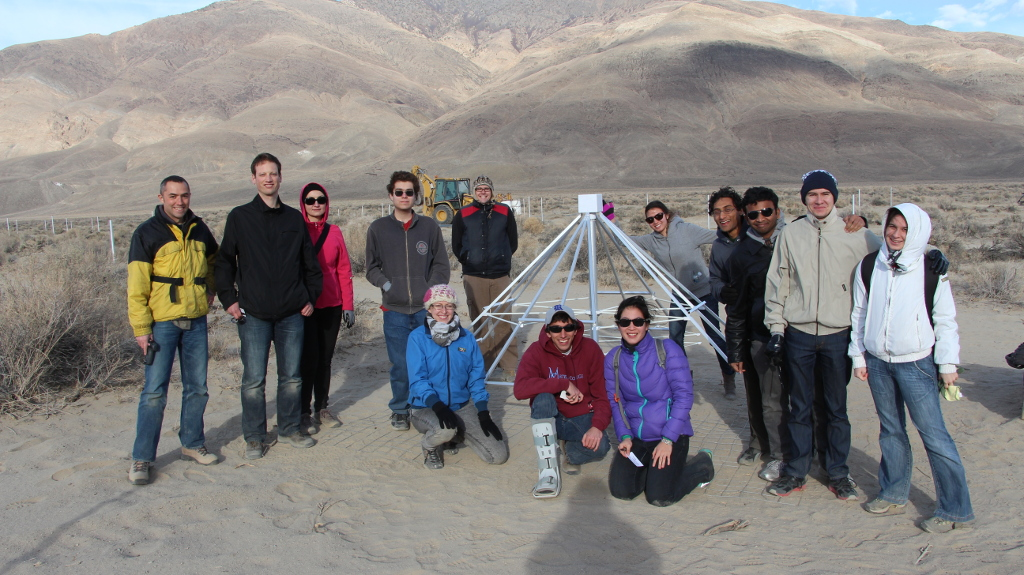
\includegraphics[width=\textwidth]{figures/chapter2/first-antenna}
    \caption{
        The first OVRO-LWA completed on 2013 March 8 with the class of Ay~122b (including the author
        of this thesis with the fractured ankle).
    }
    \label{fig:ovro-first-antenna}
\end{figure}

\begin{figure}[t]
    \centering
    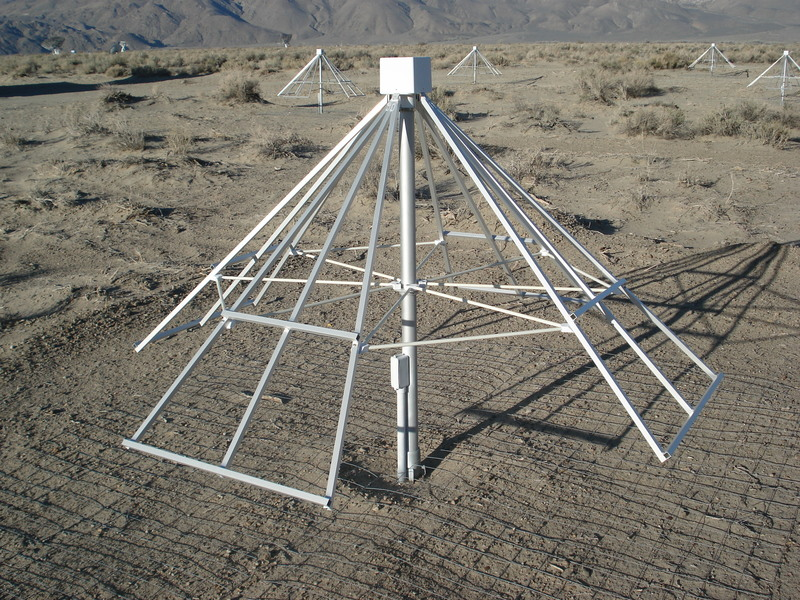
\includegraphics[width=\textwidth]{figures/chapter2/lwa-antenna}
    \caption{
        Picture of an OVRO-LWA antenna.
    }
    \label{fig:ovro-lwa-pictures}
\end{figure}

\begin{figure}[t]
    \centering
    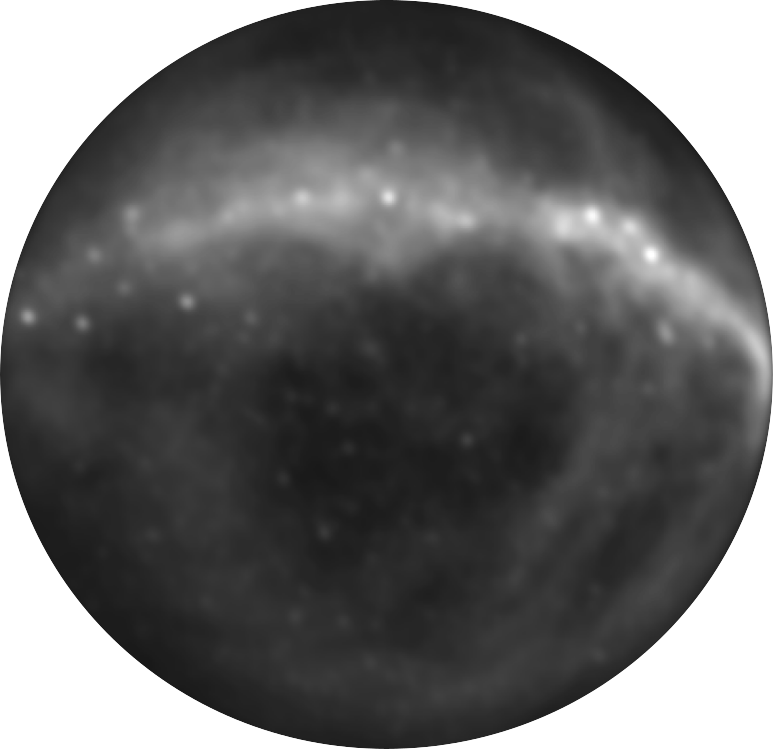
\includegraphics[width=\textwidth]{figures/chapter2/before-expansion}
    \caption{
        Snapshot image of the sky captured with the OVRO-LWA and using only the antennas located
        within the core of the array. The image covers the entire visible hemisphere in
        sine-projection.  A similar image constructed using the newer long-baseline antennas can be
        seen in Figure~\ref{fig:expansion-snapshot-image}.
    }
    \label{fig:core-snapshot-image}
\end{figure}

\begin{figure}[t]
    \centering
    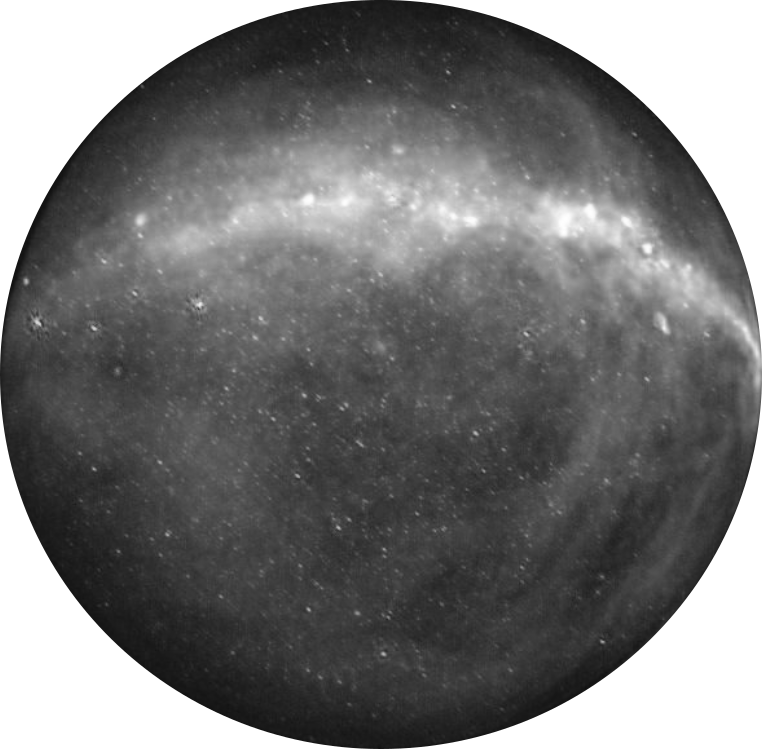
\includegraphics[width=\textwidth]{figures/chapter2/after-expansion}
    \caption{
        Snapshot image of the sky captured with the OVRO-LWA and using the new long-baseline
        antennas. The image covers the entire visible hemisphere in sine-projection.  A similar
        image constructed using only the core of the interferometer can be seen in
        Figure~\ref{fig:core-snapshot-image}.
    }
    \label{fig:expansion-snapshot-image}
\end{figure}

The OVRO-LWA is a new low-frequency (27--85\,MHz instantaneous) radio interferometer constructed
during the course of this thesis and located near Big Pine, California. Construction began in 2013
with the first antenna completed in March of that year (see Figure~\ref{fig:ovro-first-antenna}).

The OVRO-LWA was initially composed of 256 antennas, with 251 of those antennas arranged within a
dense 200\,m diameter core in a configuration that is optimized for sidelobe levels in snapshot
imaging.  Each of these antennas consists of two crossed broadband dipoles with an active
balun/preamp, and the entire system is sky noise dominated over the range 20--80\,MHz
\citep{2012PASP..124.1090H}.  A picture of an OVRO-LWA antenna can be seen in
Figure~\ref{fig:ovro-lwa-pictures}. The primary beam of each OVRO-LWA antenna subtends a solid angle
of $\sim 8000\,\text{deg}^2$, with sensitivity to the entire visible hemisphere of the sky.

\todo{ARX boards}

The remaining five antennas are isolated from the core of the OVRO-LWA and equipped with radiometric
front ends as part of the LEDA experiment, which is attempting to measure the globally averaged
signal of \ion{H}{1} from the Cosmic Dawn \citep{2018MNRAS.478.4193P}.  The OVRO-LWA hosts the LEDA
correlator as its back-end, which is an FX correlator composed of 16 ROACH2 FPGAs that compose the F
stage, and 11 servers each with dual NVIDIA K20X GPUs that compose the X stage
\citep{2015JAI.....450003K}. This allows the correlator to perform full cross-correlation of 512
input signals with 58\,MHz instantaneous bandwidth.

During observations, data is streamed from the LEDA correlator to the All-Sky Transient Monitor
(ASTM), which houses the compute nodes used for post-processing and imaging.  The ASTM is composed
of 10 identical nodes each with a 16-core Intel Xeon E5-2630 v3 CPU and 64\,GB of memory. Five
additional servers provide 565\,TB of storage capacity through the Lustre high performance file
system.

The initial 256 antenna interferometer was therefore capable of imaging the entire visible
hemisphere in snapshot images with 1$\arcdeg$ angular resolution. An example snapshot image can be
seen in Figure~\ref{fig:core-snapshot-image}.  In 2015, an additional 32 antennas were installed
that extended the maximum baseline of the interferometer to 1.5\,km and improved the angular
resolution to 8$\arcmin$. This improved angular resolution can be seen in
Figure~\ref{fig:expansion-snapshot-image}. In a final future stage of development, an additional 64
antennas will be installed that extend the maximum baseline to 2.6\,km, which will see improved
$uv$-coverage at long baselines and improved $5\arcmin$ angular resolution.

While this thesis focuses on the use of the OVRO-LWA to detect the high-redshift signature of
neutral hydrogen from the Cosmic Dawn, the OVRO-LWA facilitates a diverse set of scientific
motivations including the study of stellar and planetary magnetospheres, radio follow-up of gamma
ray bursts \citep{2017arXiv171106665A} and neutron star mergers, solar dynamic imaging spectroscopy,
and the detection of high energy cosmic rays \citep{caltechthesis11016}.

With the exception of detecting high energy cosmic rays---which uses a custom firmware and
processing pipeline that cannot operate in parallel with ordinary correlation---there are two
complementary software pipelines that service the scientific goals of the OVRO-LWA:
\begin{enumerate}
    \item A widefield snapshot imaging pipeline that images the entire visible hemisphere every
        13\,s using WSCLEAN \citep{2014MNRAS.444..606O}.
    \item A novel approach specialized for drift-scanning interferometers that can image the entire
        sky (above a limiting declination) in a single synthesis imaging step.
\end{enumerate}
This chapter will describe the calibration, source removal routines purpose built for the OVRO-LWA
and used by both pipelines. Additionally, in \S\ref{sec:commissioning-challenges} I will discuss
some of the challenges involved with commissioning the OVRO-LWA that have been overcome to bring the
OVRO-LWA into existence, to first light, and finally its first scientific results.  Finally, the
latter pipeline will be discussed in considerable depth in Chapters~\ref{chapter3} and
\ref{chapter4}.

\section{Calibration of a Low-Frequency Interferometer}

Gain calibration amounts to determining the optimal set of Jones matrices $G_i$ for each antenna $i$
such that
\begin{align}
    \b V_{ij, \text{measured}} &= \b G_i \, \b V_{ij, \text{model}} \, \b G_j^*
        + \b N_{ij} \\
    \begin{pmatrix}
        V_{ij, \text{measured}}^{xx} & V_{ij, \text{measured}}^{xy} \\
        V_{ij, \text{measured}}^{yx} & V_{ij, \text{measured}}^{yy} \\
    \end{pmatrix} &=
    \begin{pmatrix}
        g_{i}^{xx} & g_{i}^{xy} \\
        g_{i}^{yx} & g_{i}^{yy} \\
    \end{pmatrix}
    \begin{pmatrix}
        V_{ij, \text{model}}^{xx} & V_{ij, \text{model}}^{xy} \\
        V_{ij, \text{model}}^{yx} & V_{ij, \text{model}}^{yy} \\
    \end{pmatrix}
    \begin{pmatrix}
        g_{j}^{xx} & g_{j}^{xy} \\
        g_{j}^{yx} & g_{j}^{yy} \\
    \end{pmatrix}^* +
    \begin{pmatrix}
        n_{j}^{xx} & n_{j}^{xy} \\
        n_{j}^{yx} & n_{j}^{yy} \\
    \end{pmatrix}\,,
\end{align}
where $\b V_{ij,\text{measured}}$ is the Jones matrix of measured visibilities on the baseline
$i-j$, $\b V_{ij,\text{model}}$ is the Jones matrix of model visibilities (i.e., ideally what would
have been measured if the antenna and receiver did not impart any additional gain or phase), and $\b
N_{ij}$ is additional noise.

A typical calibration strategy using the Very Large Array (VLA) involves periodically pointing at a
known compact point source. For a compact point source at the phase center, the phase of all
visibilities should be zero, and the amplitude is given by the known flux (and if necessary, the
polarization) of the source.

The OVRO-LWA is capable of imaging the entire hemisphere in a snapshot image. This brings its own
unique calibration challenges because it is currently impossible to isolate a single compact point source
within the field of view of the interferometer.\footnote{
    Gated pulsar observations could, in principle, achieve this isolation. This capability is a key
    development area for the OVRO-LWA.
}
Due to the wide field of view, determining an accurate gain calibration relies on a detailed sky
and antenna beam model. Mistakes or omissions in the sky model can, for example, generate artificial
ripples in the bandpass calibration that will impact the interferometer's ability to cleanly
separate foreground emission from cosmological 21~cm emission \citep{2016MNRAS.461.3135B}.

Furthermore, at frequencies $\nu < 100\,\text{MHz}$ there are few flux calibrators.
\citet{1977A&A....61...99B} determined the absolute spectrum of Cyg~A between 20~MHz and 2~GHz.
\citet{2012MNRAS.423L..30S} added six additional calibrators, and \citet{2017ApJS..230....7P} used
the VLA 4-band system to bring the total number of available calibrators to 11. However, in
\S\ref{sec:flux-scale} I will show that the latter spectra can diverge rapidly from truth below
50~MHz.

Detailed sky and beam models are therefore generally an important calibration requirement for
low-frequency interferometers. In \S\ref{chapter3}, I derived an empirical beam model for the
OVRO-LWA and developed a new imaging formalism that captures the entire visible sky in a single
synthesis imaging step that can be used as part of a self-calibration loop.

The calibration routine itself is adapted from a variant of alternating least-squares developed by
\citet{2008ISTSP...2..707M} and \citet{2014A&A...571A..97S}. At each step this algorithm seeks to
minimize
\begin{equation}\label{eq:stefcal-step}
    \b G_i = \argmin \sum_{j \neq i}
        \left\|
            \b V_{ij, \text{measured}} - \b G_i \, \b V_{ij, \text{model}} \, \b G_j^*
        \right\|^2\,
\end{equation}
where each of the elements of $\b G_j^*$ are considered fixed. Equation~\ref{eq:stefcal-step} is
therefore a linear least-squares optimization and can be rapidly solved. However, by fixing $\b
G_j^*$ these iterations tend to oscillate about a minimum of $\chi^2$. These oscillations can be
damped by averaging subsequent iterations, and \citet{2014A&A...571A..97S} demonstrated that this
simple gradient-free optimization strategy converges remarkably quickly.

Some interferometers (e.g., HERA and the MWA), recognizing the difficulty of gain calibration at low
frequencies, have opted for partly redundant antenna configurations. These configurations can solve
for many of their calibration parameters internally without relying on an incomplete sky model and
potentially inaccurate antenna beam model \citep{2010MNRAS.408.1029L}. However, these
interferometers sacrifice imaging fidelity, which is useful for establishing the remaining
calibration parameters (e.g., the overall bandpass cannot be solved for in an internal
redundant-calibration routine).\footnote{
    The HERA collaboration is currently investigating the possibility of determining the overall
    bandpass through redundancies between frequency channels. The author of this thesis is not
    optimistic about this approach.
}

\section{Source Removal and Direction-Dependent Calibration}

Because the OVRO-LWA antenna layout is optimized for sidelobe levels in snapshot imaging, the
point-spread function (PSF) is pretty good.

\section{Commissioning Challenges}
\label{sec:commissioning-challenges}

\subsection{Computing Antenna Positions}

\begin{figure}
    \centering
    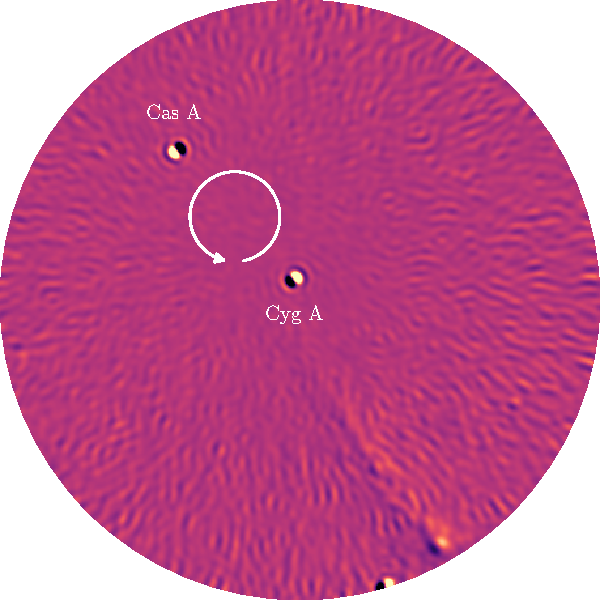
\includegraphics[width=\textwidth]{figures/chapter2/northing-easting-mistake/northing-easting-mistake}
    \caption{
        Illustration of the error in the WCS prior to a correction to the antenna positions. The
        image is a difference between an image constructed with the incorrect antenna positions and
        the corrected antenna positions. The arrow denotes the direction and approximate center of
        the rotation.
    }
    \label{fig:northing-easting-mistake}
\end{figure}

Early images produced by the OVRO-LWA (prior to 2015 October 16) were afflicted by an apparent
rotation in the World Coordinate System (WCS).

\subsection{RFI Localization}

\begin{figure}
    \centering
    \begin{tabular}{cc}
        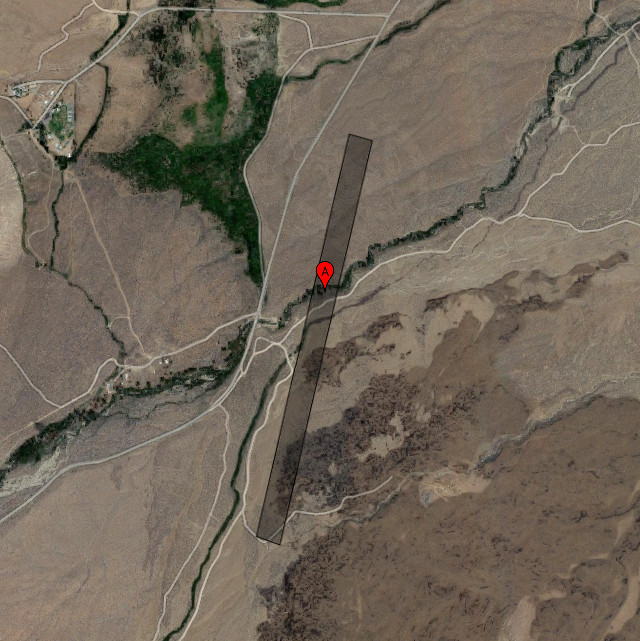
\includegraphics[width=0.45\textwidth]{figures/chapter2/google-maps-rfi-localization} &
        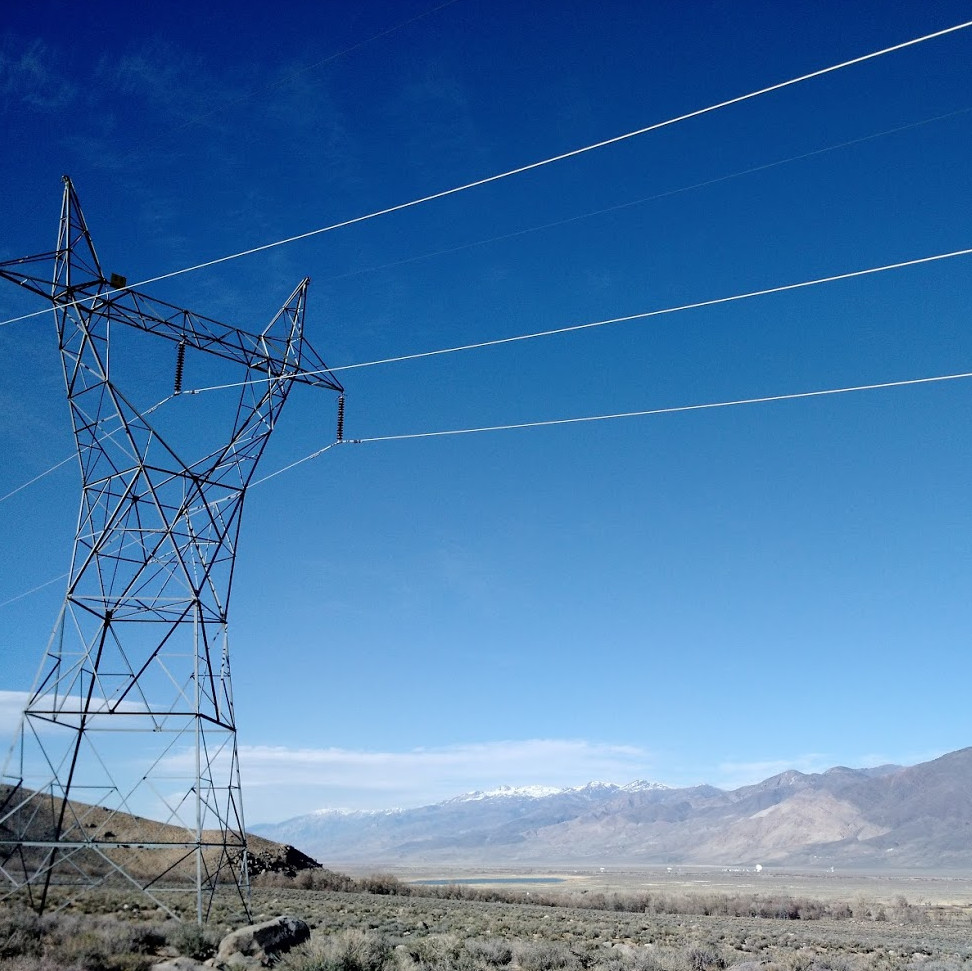
\includegraphics[width=0.45\textwidth]{figures/chapter2/power-line-picture} \\
        (a) & (b) \\
    \end{tabular}
    \caption{
        (a) The localization region for a source of RFI south of the OVRO-LWA and near the town of
        Big Pine. Satellite imagery \textcopyright2018 Google. Map data \textcopyright2018 Google.
        (b) Image of a high-voltage power line overlooking OVRO near the localization region.
    }
    \label{fig:rfi-localization}
\end{figure}

An ongoing challenge faced by the OVRO-LWA is the presence of broadband sources of RFI in the
vicinity of the observatory. Due to the entire-hemisphere field of view of the OVRO-LWA, these
sources appear as points on the horizon that limit the sensitivity of snapshot images through
additional sidelobe noise. Fortunately, because these sources are typically in the near-field of the
interferometer, the curvature of the incoming wavefront can be used to infer the distance to each
source of RFI.

The path difference from a source in the near-field of an interferometer located at the position
$(\xi, \eta, \zeta)$ to two antennas located respectively at $(x_i, y_i, z_i)$ and $(x_j, y_j, z_j)$
is
\begin{equation}\label{eq:nearfield-path-difference}
    \Delta l^\text{near-field}_{ij} =
        \sqrt{(x_j - \xi)^2 + (y_j - \eta)^2 + (z_j - \zeta)^2}
        - \sqrt{(x_i - \xi)^2 + (y_i - \eta)^2 + (z_i - \zeta)^2}\,.
\end{equation}
In the limit that the distance of the source goes to infinity, we recover the familiar expression
\begin{equation}\label{eq:farfield-path-difference}
    \Delta l^\text{far-field}_{ij} = \frac{1}{D}\Big(
        (x_i - x_j)\,\xi + (y_i - y_j)\,\eta + (z_i - z_j)\,\zeta
    \Big)\,,
\end{equation}
where $D$ is the distance to the source. The correlation measured between two antennas for a source
in the near-field of the interferometer is therefore
\begin{equation}\label{eq:nearfield-visibilities}
    V_{ij} = F \exp\left(2\pi i \frac{\Delta l^\text{near-field}_{ij}}{\lambda}\right)\,,
\end{equation}
where $V_{ij}$ is the visibility measured between antennas $i$ and $j$, $F$ is the apparent
brightness of the source, and $\lambda$ is the wavelength. Equation~\ref{eq:nearfield-visibilities}
can then be used to fit for the position of a source including its distance.

In order to improve sensitivity to these RFI sources,



\myputbib{thesis}
\end{bibunit}

